\subsubsection{Control de señales críticas}

El SAL/T debe tener la capacidad de controlar directamente las señales críticas de control de tracción (CT) y freno de emergencia (FE). Estas señales son las más críticas que interactúan con el sistema, ya que pueden controlar el movimiento de la formación, bloquearla o permitirle el avance ignorando el estado de todos los SIS. Por estos motivos, se implementó un circuito redundado de mayor seguridad para la activación y corte de estas señales; uno para la señal de CT y otro para la señal de FE como ya se explicó que trabajan con líneas independientes. Este circuito reutiliza los conceptos del prototipo anterior explicados en su informe \cite{salt_ivan}.  \\ 

El circuito de control de las señales críticas cuenta con dos entradas y una salida. Una entrada es la línea de la señal crítica después de haber pasado por las llaves interruptoras de los distintos SIS y de los circuitos de aislamiento de estos (IN); la otra entrada es una alimentación provista por la formación capaz de energizar la electroválvula (ACT); se espera una tensión de entre 72 V y 110 V acorde a la tensión de las baterías del tren; pero al trabajar con relés, solo se va a conectar o desconectar esta señal de la línea y no se va a trabajar en su procesamiento. La salida (OUT) va directamente a la conexión con la electroválvula. En la figura \ref{fig:rele_seguridad} se observa cómo es la configuración del sistema de activación de una señal crítica respecto a los interruptores de los SIS y sus sistemas de aislamiento (expuesto de manera simplificada) y respecto a la electroválvula de la señal crítica; también se muestra el arreglo de tres relés con sus respectivas entradas y salidas mencionadas. 

\begin{figure}[H]
    \centering
    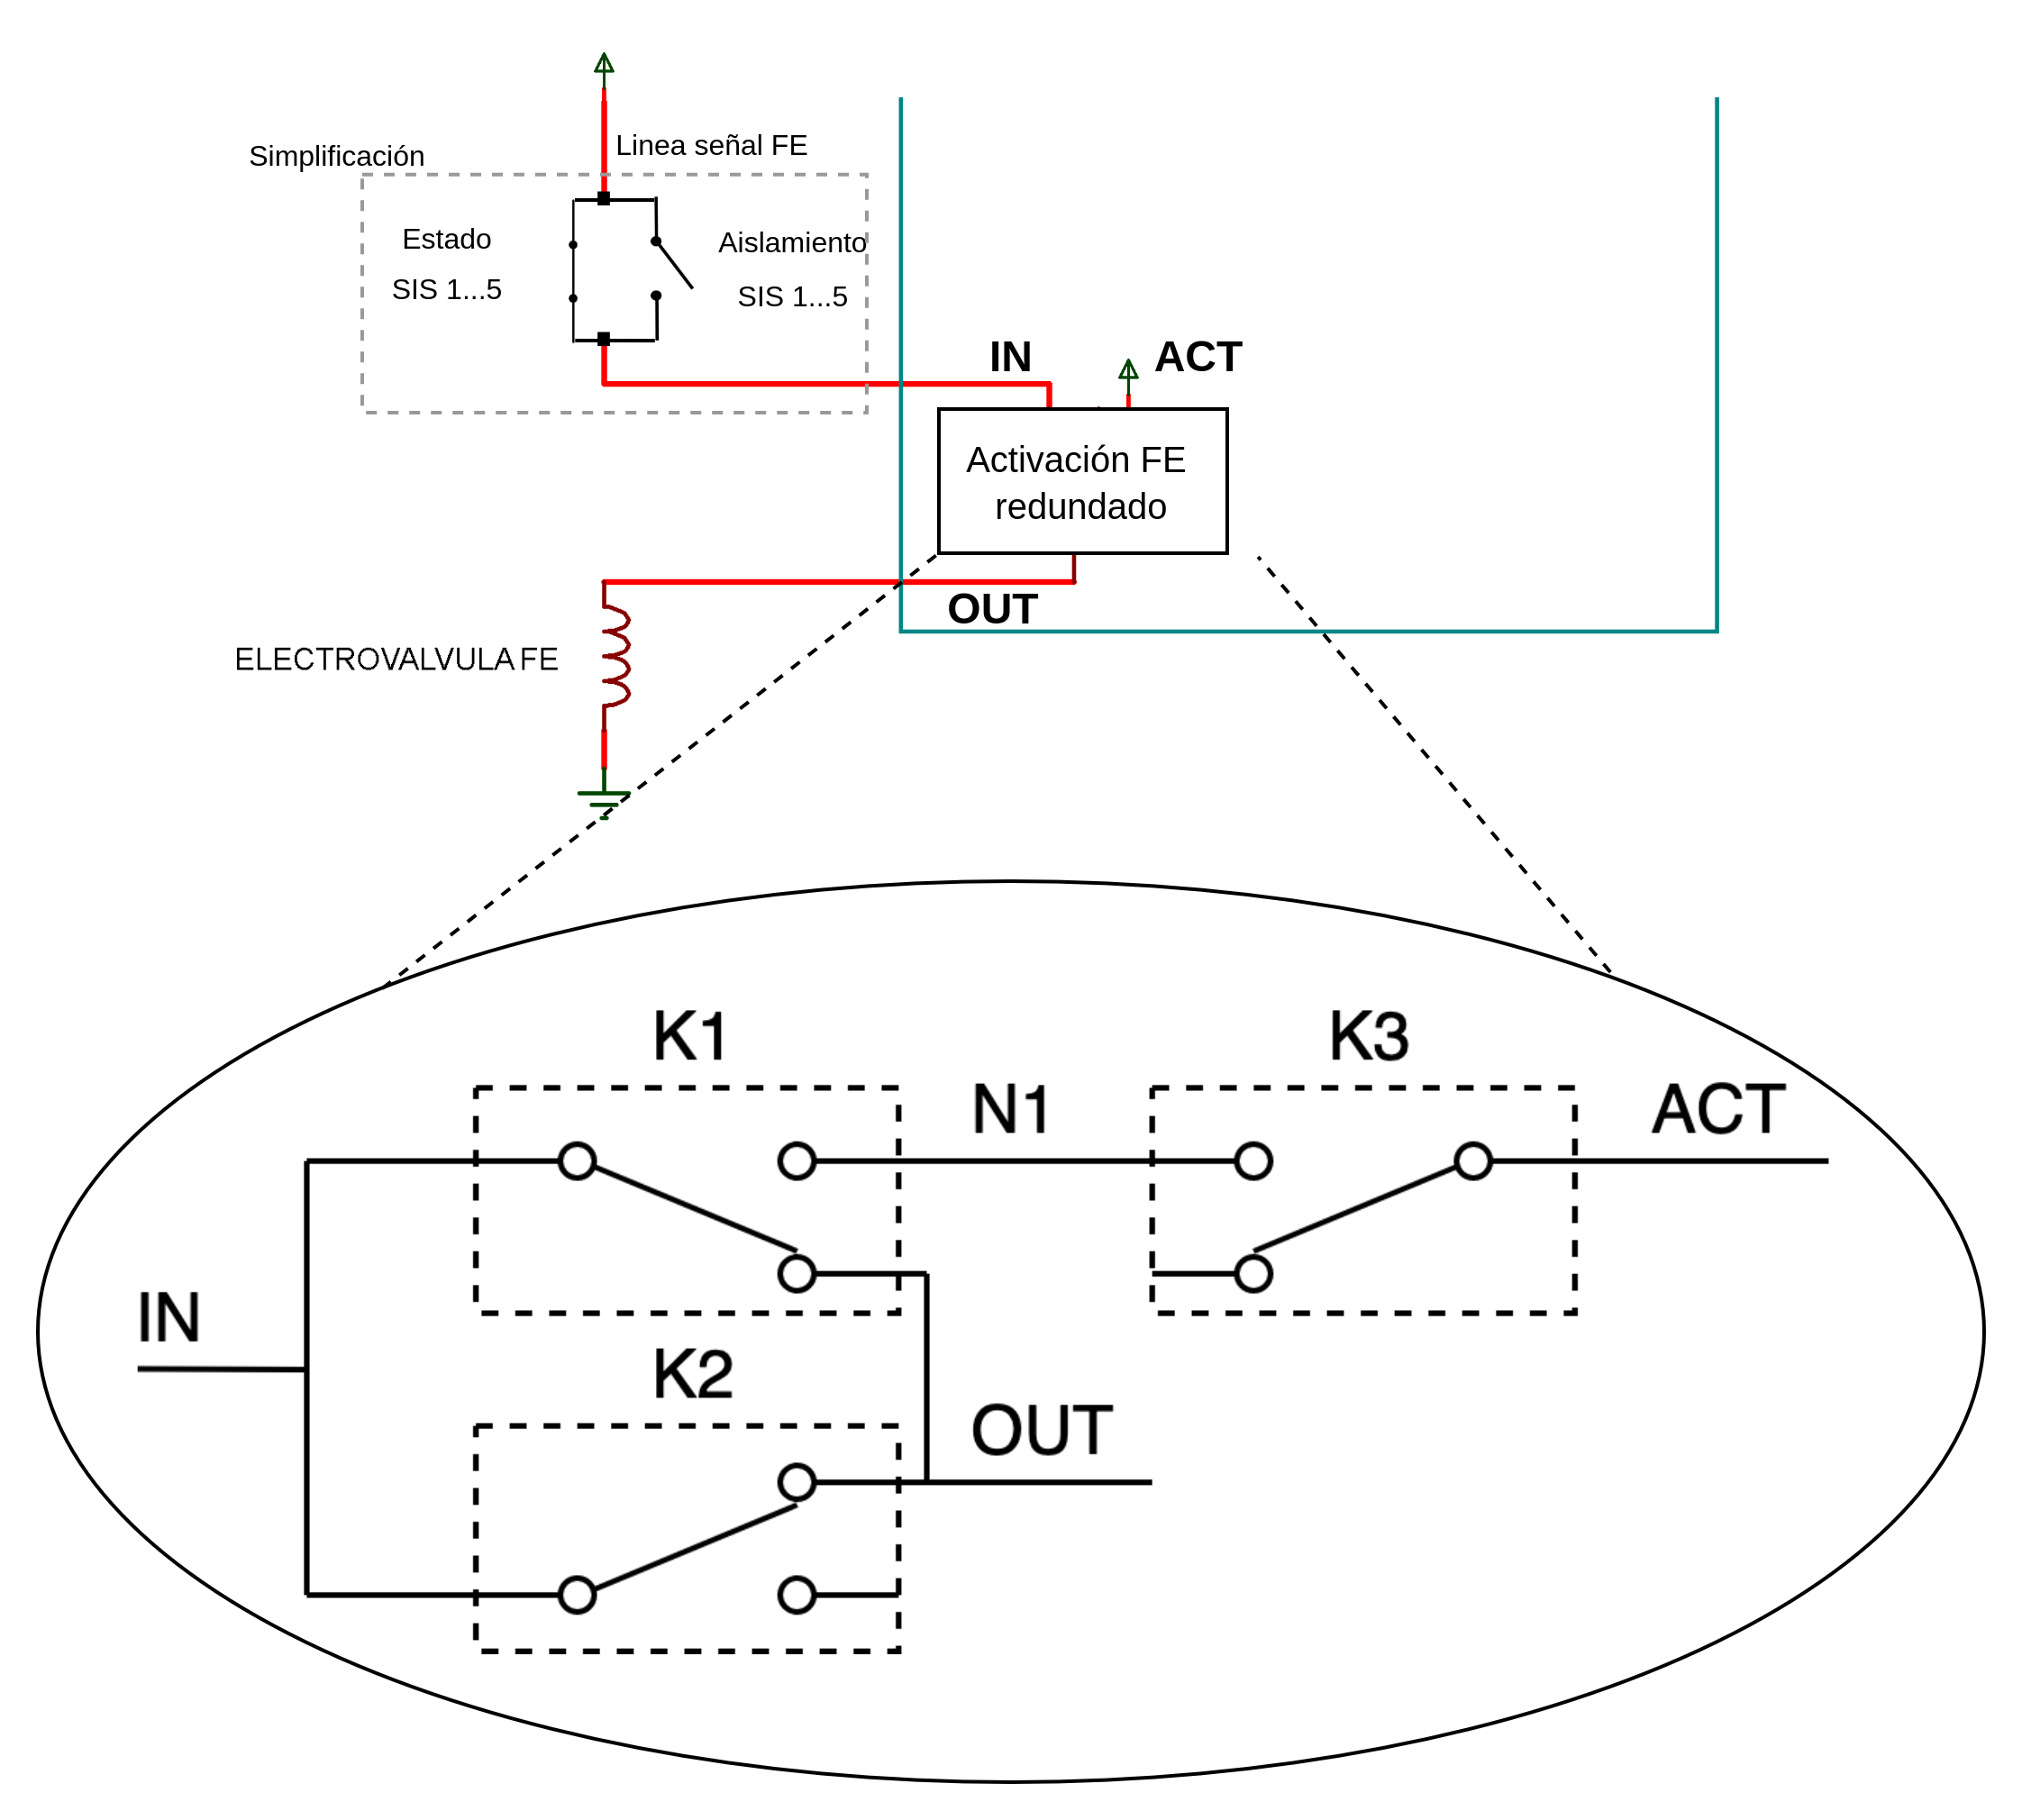
\includegraphics[width = \linewidth]{img/reles_critico.png}
    \caption{Circuito de relés redundado para activación de señales críticas}
    \label{fig:reles_critico}
\end{figure}

Para estos relés, se utilizó el mismo modelo que para el aislamiento de los SIS (JW2SN-DC5V) pero con la misma consideración de que sirven de reemplazo para relés de seguridad de las mismas características de contactos. Para alimentar estos relés, se utilizó un nuevo driver de potencia ULN2003 que permite activar los seis relés (tres para CT y tres para FE) de estos circuitos. \\ 

Los estados del circuito se pueden resumir de la siguiente manera:

\begin{itemize}
    \item \textbf{Estado normal}: el circuito no modifica la línea de la señal crítica. La entrada IN queda conectada directamente con OUT. La señal de ACT no interviene en la línea. Este estado no realiza ninguna modificación respecto a la línea tradicional sin el SAL/T y debe asegurarse que, ante una falla en el sistema, se imponga este estado dejando la activación de la señal crítica controlada por los SIS. 

    \item \textbf{Activación señal crítica o circuito abierto}: la salida OUT queda desconectada de las entradas IN y ACT. De esta manera, se asegura que el circuito queda abierto y la electroválvula quede sin alimentación lo que fuerza que la señal crítica se ejecuta. Este estado debe forzarse cuando se desea detener la formación activando el freno de emergencia o anulando el control de tracción. 

    \item \textbf{Alimentación forzada o \textit{bypass}}: la salida OUT se conecta directamente con la entrada ACT. De esta manera, la electroválvula queda alimentada independientemente de la tensión en IN y del estado de los SIS de la línea. Este estado es el más crítico porque desactiva todos los SIS de la formación y le permite el movimiento en este estado inseguro. 

\end{itemize}

Para forzar los estados mencionados, se deben controlar los relés considerando que la figura \ref{fig:reles_critico} muestra el estado normal (desenergizado) de cada uno de ellos de acuerdo a la tabla \ref{tab:estado_rele}.

\begin{table}[htb]


    \begin{tabular}{|c|c|} 
        \hline
        \textbf{Estado del circuito} & \textbf{Posición de los relés}\\
        \hline
        Estado normal     &     K1, K2 y K3 desenergizados   \\
        \hline
        Circuito abierto   &     K1 y K2 energizados. K3 desenergizado   \\
        \hline
        \textit{Bypass}   &     K1 y K3 energizados. K2 desenergizado   \\
        \hline
    \end{tabular}
\caption{Posición de relés para los estados del circuito redundado}
\label{tab:estado_rele}
\end{table}

Este sistema aumenta la seguridad de las conexiones, ya que los relés K1 y K2 cumplen una función de redundancia para volver al estado normal. En caso de que alguno de los tres relés falle, esto significa que quede pegado en una posición no deseada, se pueden utilizar los otros dos relés para asegurarse de volver al estado normal donde IN está conectado con OUT. Por ejemplo, si el relé K1 falla y queda pegado conectado al nodo N1, la conexión entre IN y OUT va a seguir existiendo y no se va a generar ningún problema mientras K3 esté desenergizado. Si K2 falla, K1 conecta directamente IN y OUT. Si K3 falla, se mantiene el estado normal, ya que el nodo N1 no participa de este estado. \\ 

Al utilizar relés con dos salidas, una para este circuito de activación y otra para la medición del estado del relé, se puede detectar en todo momento cuando un relé quedó en un estado incorrecto y forzar al SAL/T en un estado de error interno restaurando la conexión normal de las señales críticas. 
